\documentclass[dvipsnames]{beamer}
\usepackage{lmodern}
\usepackage{appendixnumberbeamer}
\renewcommand{\sfdefault}{lmss}
\renewcommand{\ttdefault}{lmtt}
\usepackage[T1]{fontenc}
% \usepackage[utf8]{inputenc}
\setcounter{secnumdepth}{3}
\setcounter{tocdepth}{3}
\usepackage{amsmath}
\usepackage{amsthm}
\usepackage{amssymb}
\theoremstyle{definition}
\newtheorem*{defn*}{\protect\definitionname}
\providecommand{\definitionname}{Definition}
\usepackage{graphicx}
\usepackage{hyperref}
\usepackage{ulem}
\PassOptionsToPackage{normalem}{ulem}
\usepackage{caption}
\usepackage{subcaption}
\usepackage{verbatim}
\usepackage[english]{babel}
\usepackage[autostyle]{csquotes}
\usepackage{tikz}
\usetikzlibrary{arrows,intersections}
\usepackage{pgfplots}
\pgfplotsset{compat = 1.15}
\usepgfplotslibrary{fillbetween}
\usepackage{verbatim}
\usepackage{booktabs}
\usepackage{multirow}
\usepackage{array}
\usepackage{nccmath}
% \usepackage{listings}
\usepackage{mathtools}

%Bibliography style, etc.
\usepackage[citestyle=authoryear-comp,natbib, uniquename = false, url = false, doi = false, uniquelist=false]{biblatex}
\renewbibmacro{in:}{}
\AtEveryBibitem{%
  \clearfield{volume}%
  \clearfield{number}
  \clearfield{month}
  \clearfield{issn}
  \clearfield{isbn}
  \clearfield{pages}
}

%\usepackage{cleveref}
\usepackage{setspace}
\makeatletter

% Macros
\providecommand{\tabularnewline}{\\}
\newcommand{\gr}{\textcolor{ForestGreen}} 
\newcommand{\rd}{\textcolor{red}}
\newcommand{\cb}{\textcolor{CornflowerBlue}} %this is the blue color you like; simply type \cb{X} where "X" is the color you want in blue
\newcommand{\vitem}{\vfill \item} %auto-centers items in lists
\newcommand{\fall}{\ \forall} %redefines "forall" (I don't like the default spacing)
\newcommand{\frall}{\quad \forall} %a \forall separated from the main math; this is the way it usually shows up in equations
\newcommand{\exist}{\ \exists} %same as \fall, but for \exists; they have the same ugly spacing
\newcommand{\R}{\mathbb{R}} %set of real numbers
\newcommand*\bigcdot{\mathpalette\bigcdot@{.5}} %different size for cdots
% \newcommand{\argmax}{\text{arg}\max}
\newenvironment{itemframe}
    {\frame{}\itemize}
    {\itemize\frame}
\newcommand\makebeamertitle{\frame{\maketitle}}%
\newtheoremstyle{named}{}{}{\itshape}{}{\bfseries}{.}{.5em}{\thmnote{#3's }#1}
\theoremstyle{named}
\newtheorem*{prop*}{Proposition}
% \newtheorem*{corollary}{Corollary}
\newtheorem*{namedtheorem}{Theorem} %allows named theorems
\newtheorem*{nameddef}{Definition}
\newtheorem{proposition}{Proposition}
\newtheorem*{assumption}{Assumption}
\newtheorem*{namedcorollary}{Corollary}
\newtheorem*{namedlemma}{Lemma}
\newtheorem*{axiom}{Axiom}
\newtheorem*{theorem*}{Theorem}
\newtheorem*{lemma*}{Lemma}
\DeclareMathOperator*{\argmin}{argmin}
\DeclareMathOperator{\argmax}{argmax}
\DeclareMathOperator{\supp}{supp}
\DeclareMathOperator{\interior}{int}
\DeclareMathOperator{\rank}{rank}
\newcolumntype{C}[1]{>{\centering\let\newline\\\arraybackslash\hspace{0pt}}m{#1}}
\newcommand{\sbt}{\,\begin{picture}(-1,1)(-1,-3)\circle*{2}\end{picture}\ }



%formatting
\usetheme{Ilmenau}
\definecolor{MIT}{rgb}{.639,.122,.204}
\definecolor{UCLA}{rgb}{0.15294117647058825, 0.4549019607843137, 0.6823529411764706}
\definecolor{UCLA_gold}{rgb}{1, 0.8196078431372549, 0}
\usecolortheme[named=UCLA]{structure}
\setbeamercolor*{palette secondary}{fg=UCLA_gold,bg=gray!15!white}
\usecolortheme{dolphin}
\setbeamertemplate{navigation symbols}{} 
\setbeamertemplate{footline}{}{}
\setbeamertemplate{headline}{}
\setbeamertemplate{navigation symbols}{}
\mode<presentation> {}
\setbeamercolor{block title}{use=structure,fg=white,bg=RoyalBlue} %blocks (theorems, etc.)in blue
\setbeamercolor{block title alerted}{use=structure,fg=white,bg=ForestGreen} %blocks (theorems, etc.)in blue

\renewcommand\qedsymbol{$\blacksquare$} %set QED symbol as black square
\renewcommand{\emph}{\textit} %set emphasized text style; this is italics
\setbeamertemplate{footline}[frame number] %slide numbers
\setbeamertemplate{itemize item}[circle] %bullet style
\setbeamertemplate{itemize subitem}{--}
\setbeamertemplate{enumerate item}[default]
\newrobustcmd*{\parentexttrack}[1]{%
  \begingroup
  \blx@blxinit
  \blx@setsfcodes
  \blx@bibopenparen#1\blx@bibcloseparen
  \endgroup}

\AtEveryCite{%
  \let\parentext=\parentexttrack%
  \let\bibopenparen=\bibopenbracket%
  \let\bibcloseparen=\bibclosebracket}

 \AtBeginDocument{%
   \let\origtableofcontents=\tableofcontents
   \def\tableofcontents{\@ifnextchar[{\origtableofcontents}{\gobbletableofcontents}}
   \def\gobbletableofcontents#1{\origtableofcontents}
 }
\newcommand{\backupbegin}{
   \newcounter{framenumberappendix}
   \setcounter{framenumberappendix}{\value{framenumber}}
}
\newcommand{\backupend}{
   \addtocounter{framenumberappendix}{-\value{framenumber}}
   \addtocounter{framenumber}{\value{framenumberappendix}} 
} 

\renewcommand{\maketitle}{
\setbeamertemplate{footline}{} 
\begin{frame}[noframenumbering]
\titlepage
\end{frame}
\setbeamertemplate{footline}[frame number]
}

\usefonttheme[onlymath]{serif}

% \usetheme{CambridgeUS}

% \newtheorem{theorem}{Theorem}
% \theoremstyle{claim}
\newtheorem{claim}{Claim}
% \newtheorem{corollary}{Corollary}


\makeatother


%\author{Drew Fudenberg}

\institute[]{}
\title{Competition Under Social Interactions and the Design of Education Policies}
\author{Claudia Allende \\[2em] \small{This presentation prepared for UCLA Econ 272A by Chris Ackerman.}}
\begin{document}
\maketitle

\begin{frame}{Overview}
  \begin{itemize}
  \item[Question:] Model the education market in Peru 
    \begin{itemize}
    \item What happens when students/families have preferences over their peers?
    \end{itemize}
    \vitem[Approach:] BLP with schools' shares of local education markets
    \begin{itemize}
    \item Include (expected) peer quality in students' valuations of schools
    \end{itemize}
    \vitem[Results:] Firms have more market power but do not mark down quality by as much when accounting for social interactions
    \begin{itemize}
    \item The ``best'' policy from an equity/efficiency perspective is a combination of targeted vouchers and land lease subsidies
    \end{itemize}
  \end{itemize}
\end{frame}
%
\begin{frame}{Motivation---Why include social interactions?}
  \begin{center}
   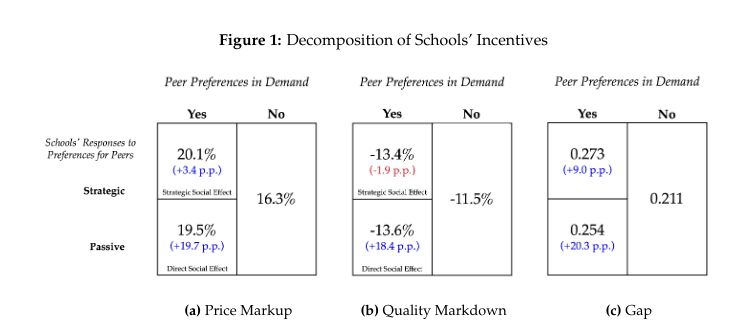
\includegraphics[width=\textwidth, keepaspectratio=true]{figs/fig1.png} 
  \end{center}
\end{frame}
%
\begin{frame}{Empirical Setting---First Graders in Peru}
  \begin{itemize}
  \item Since 1998 there has been basically free entry (anyone can start a school)
    \vitem Teacher compensation reform in 2012
    \begin{itemize}
    \item Use this to generate variation in wages across both time and locations
    \end{itemize}
    \vitem School admissions reform in 2012
    \begin{itemize}
    \item No more price discrimination
      \item No more active selection/discrimination against students
    \end{itemize}
    \vitem Teachers strike at Public Schools in 2017
    \begin{itemize}
    \item Use this to generate an IV later in the paper
    \end{itemize}
  \end{itemize}
\end{frame}
%
\begin{frame}{Model---Timing}
  \begin{center}
   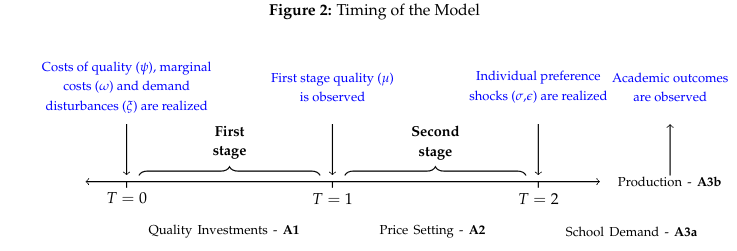
\includegraphics[width=\textwidth, keepaspectratio=true]{figs/fig2.png} 
  \end{center}
  \begin{enumerate}
  \item Schools see their costs, choose a quality
    \vitem Schools observe quality and choose prices to maximize profits
    \vitem Individuals have preferences for schools; select the best school based on their expected peer quality
    \vitem Students go to school, interact with each other, and have education outcomes
  \end{enumerate}
\end{frame}
%
\begin{frame}{School Value-Added}
  \[
 Y_{i j t}(\tau)=\mathbf{X}_{i t}^{\prime} \pi^{x}+\theta_{j t}(\tau)+\epsilon_{i j t} 
 \]
 \begin{itemize}
 \item $\theta_{ij}(\tau)$ is value-added; common for all students
   \begin{itemize}
   \item $\tau$ only important for counterfactuals
   \end{itemize}
   \vitem $x_i = (x_i^y, x_i^e)$ indicates high income/human capital
   \vitem $\mathbf{z}_{jt}$ includes the mean for $x_i$ for school $j$ at time $t$
 \end{itemize}
\end{frame}
%
\begin{frame}{Decomposing Value-Added}
  \[
\theta_{j t}(\tau)=\mathbf{z}_{j t}(\tau)^{\prime} \pi^{z}+\underbrace{\mathbf{I}_{\mathbf{j t}}(\tau)^{\prime} \pi^{1}(\tau)+\epsilon_{j t}^{s}(\tau)}_{\mu_{j t}(\tau)}
  \] 
  \begin{itemize}
  \item $\mu_{ij}(\tau)$ is observable school quality
    \begin{itemize}
    \item Does not try to break out the different components of $\mu$; claims it is sufficient to have a measure of $\mu$
    \end{itemize}
    \vitem The peer-effects have three components:
    \begin{enumerate}
    \item Direct effect of student characteristics on outcomes
      \vitem Direct effect of peer characteristics on outcomes
      \vitem Indirect effects of school composition on outcomes
      \begin{itemize}
      \item For example, easier to hire good teachers if the school is full of well-behaved students
      \end{itemize}
    \end{enumerate}
  \end{itemize}
\end{frame}
%
\begin{frame}{Demand for Schools}
  Schools have the following relevant characteristics:
  \begin{itemize}
  \item Quality: $\mu_{jt}$
    \vitem Price: $p_{jt}$
    \vitem Student body characteristics: $z_{jt}^y, z_{jt}^e$
    \vitem Location: $loc_j$
    \vitem Private voucher network status: $net_{jt} = \mathbf{1}(j \in \Omega_{network})$
    \vitem Vector of other characteristics (religious status, etc.): $r_{jt}^\prime$
  \end{itemize}
\end{frame}
%
\begin{frame}{Demand for Schools}
  \[
U_{i j t}=\beta_{i}^{\mu} \mu_{j t}-\alpha_{i} p_{j t}+\beta_{i}^{z^{y}} \hat{z}_{j t}^{y}+\beta_{i}^{z^{e}} \hat{z}_{j t}^{e}+\beta_{i}^{d} D_{i j}+\beta_{i}^{n e t} n e  t_{j t}+r_{j t}^{\prime} \beta^{r}+\xi_{j t}+\epsilon_{i j t}
% \\[.5em]
% \text{Where}
  \]
  \begin{itemize}
  \vitem Utility is over the \emph{expectation} for student body composition
    \vitem Preference for quality and student body composition are heterogeneous along unobserved family characteristics
  \end{itemize}
  \[
\alpha_{i}=\bar{\alpha}+\sum_{l=y, e} \alpha_{l} x_{i}^{l}, \quad \text { same for } \beta_{i}^{d}
\\[.5em]
\beta_{i}^{\mu}=\bar{\beta}^{\mu}+\sum_{l=y, e} \beta_{l}^{\mu} x_{i}^{l}+\beta_{u}^{\mu} v_{i}, \quad \text{same for} \beta_{i}^{z^{y}}$ and $\beta_{i}^{z^{e}}, \quad
\\[.5em]
\hspace{-2em}  v_{i} \sim \ln \mathcal{N}\left(m_{v}, \Sigma\right), \quad
\beta_{i}^{\text {net }}=\bar{\beta}^{\text {net }}+\sigma^{\text {net }} v_{i}^{\text {net }}, \quad \text { with } v_{i}^{\text {net }} \sim \mathcal{N}(0,1)
  \]
\end{frame}
%
\begin{frame}{Beliefs about student body composition}
  \begin{itemize}
  \item Families form beliefs that are consistent with the expectation of the realized student body composition of the school
    \vitem $z^y$ and $z^e$ satisfy the system of equations
    \[
\hspace{-3em}\resizebox{\textwidth}{!}{\mathcal{Z}_{j t}^{x}\left(\mu, \mathbf{p}, \mathbf{z}^{y}, \mathbf{z}^{e}\right)=\frac{N \times \pi_{k=x}^{m} \times \sum_{n}^{N_{m}} \sum_{i}^{N_{v}} \mathcal{S}_{i j t}^{n, k=x}\left(\mu, \mathbf{p}, \mathbf{z}^{y}, \mathbf{z}^{e}\right) \times w^{v} \times w_{n, k=x}^{m}}{N \times \sum_{k}^{K} \sum_{n}^{N_{m}} \sum_{i}^{N_{v}} \mathcal{S}_{i j t}^{n k}\left(\mu, \mathbf{p}, \mathbf{z}^{y}, \mathbf{z}^{e}\right) \times w^{v} \times w_{n k}^{m} \times \pi_{k}^{m}}}
\]

For $x=\{y, e\}$ and $j=\left\{1, \ldots, N_{j}^{m}\right\}$
  \end{itemize}
\end{frame}
%
\begin{frame}{BLP share equations}
  \begin{itemize}
  \item Assume $\epsilon_{ijt}$ has an EV distribution; the probability that a type-$k$ family living at node $n$ with unobservable type $v_i$ selects school $j$ is
    \[
\mathcal{S}_{i j t}^{n k}\left(\mu, \mathbf{p}, \mathbf{z}^{y}, \mathbf{z}^{e}\right)=\left(\frac{\exp \left(U_{i j t}\left(\mu, \mathbf{p}, \mathbf{z}^{y}, \mathbf{z}^{e}\right)\right)}{\sum_{l \in \Omega_{i t}} \exp \left(U_{i l t}\left(\mu, \mathbf{p}, \mathbf{z}^{y}, \mathbf{z}^{e}\right)\right)}\right)
    \]
    \vitem We can aggregate across individuals to get market-level shares,
    \[
\begin{gathered}
s_{j t}^{k}\left(\boldsymbol{\mu}, \mathbf{p}, \mathbf{z}^{y}, \mathbf{z}^{e}\right)=\sum_{n}^{N_{m}} s_{j t}^{n k} \cdot w_{n k}^{m} \\
s_{j t}\left(\boldsymbol{\mu}, \mathbf{p}, \mathbf{z}^{y}, \mathbf{z}^{e}\right)=\sum_{k}^{K} \sum_{n}^{N_{m}} s_{j t}^{n k} \cdot w_{n k}^{m} \cdot \pi_{k}^{m}
\end{gathered}
    \]    
  \end{itemize}
\end{frame}
%
\begin{frame}{Supply---Costs}
  \[
M C_{j}\left(\mu_{j t}\right)=\sum_{l} \gamma_{l} w_{j t}^{l}+\gamma_{\mu} \mu_{j t}+\omega_{j t}
  \]
  \[
F C_{j}\left(\mu_{j t}\right)=\sum_{l} \lambda_{l} w_{j t}^{l}+\psi_{j t} \mu_{j t \prime \prime} \quad \text { where } \psi_{j t}=\bar{\psi}_{j}+\Delta \psi_{j t}
  \]
  \begin{itemize}
  \item $\omega_{jt}$ is the unobserved part of marginal cost
    \vitem $\psi_{jt}$ is the fixed cost of providing quality $\mu_{jt}$
    \begin{itemize}
     \item Persistent component $\overline{psi}_j$ and shock $\Delta \psi_{jt}$ 
    \end{itemize}
  \end{itemize}
\end{frame}
%
\begin{frame}{Second Stage---Pricing Decision}
  \[
\pi_{j t}\left(\mu, \mathbf{p}, \mathbf{z}^{y}(\mathbf{p}), \mathbf{z}^{e}(\mathbf{p})\right)=\left(p_{j t}-M C_{j t}\left(\mu_{j t}\right)\right) \times N \times s_{j t}\left(\mu, \mathbf{p}, \mathbf{z}^{y}(\mathbf{p}), \mathbf{z}^{e}(\mathbf{p})\right)-F C_{j t}\left(\mu_{j}\right)
  \]  
  \[
p_{j t}^{*}=\underbrace{\sum_{l} \gamma_{l} w_{j t}^{l}+\gamma_{\mu} \mu_{j t}+\omega_{j t}}_{\text {Marginal Cost }}+\underbrace{s_{j t} \times\left(-\frac{d s_{j t}\left(\mu, \mathbf{p}, \mathbf{z}^{y}(\mathbf{p}), \mathbf{z}^{e}(\mathbf{p})\right)}{d p_{j t}}\right)^{-1}}_{\text {Price Markup with Social Interactions }}
  \]
  \begin{itemize}
  \item Pricing equation accounts for the effects social interactions have on the school's pricing strategy
    \vitem Considers both the direct and strategic effects of including $z^y(p)$ and $z^e(p)$ in demand
  \end{itemize}
\end{frame}
%
\begin{frame}{Incentives---Individual Demand}
  \begin{align*}
    \frac{d s_{i j t}}{d p_{j t}}&=\underbrace{\overbrace{\frac{\partial s_{i j t}\left(\boldsymbol{\mu}, \mathbf{p}, \mathbf{z}^{y}(\mathbf{p}), \mathbf{z}^{e}(\mathbf{p})\right)}{\partial p_{j t}}}^{\text {Sensitivity to price - (a) }}}_{\text {I - Direct Effect (Baseline + Social) }}\\[1em]
                                 &+\sum_{l \in \Omega_{i t}} \overbrace{\frac{\partial s_{i j t}\left(\boldsymbol{\mu}, \mathbf{p}, \mathbf{z}^{y}(\mathbf{p}), \mathbf{z}^{e}(\mathbf{p})\right)}{\partial z_{l t}^{y}}}^{\text {Sensitivity to peers (Poor) - (b) }} \times \overbrace{\frac{d z_{l t}^{y}\left(\boldsymbol{\mu}, \mathbf{p}, \mathbf{z}^{y}(\mathbf{p}), \mathbf{z}^{e}(\mathbf{p})\right)}{d p_{j t}}}^{\text {Change in peers (Poor) - (c) }}\\[1em]
    &\underbrace{+\sum_{l \in \Omega_{i t}} \frac{\overbrace{\partial s_{i j t}\left(\boldsymbol{\mu}, \mathbf{p}, \mathbf{z}^{y}(\mathbf{p}), \mathbf{z}^{e}(\mathbf{p})\right)}^{\text {Sensitivity to peers (M.Educ) - (d) }}}{\partial z_{l t}^{e}} \times \frac{\overbrace{d z_{l t}^{e}\left(\boldsymbol{\mu}, \mathbf{p}, \mathbf{z}^{y}(\mathbf{p}), \mathbf{z}^{e}(\mathbf{p})\right)}^{\text {Change in peers (M.Educ) - (e) }}}{d p_{j t}}}_{\text {II - Strategic Social Effect }}
  \end{align*} 
\end{frame}
%
\begin{frame}{Incentives---Individual Demand}
  \begin{itemize}
  \item Term (I) is the direct effect of prices on demand
    \vitem Second term is the strategic social effect of prices on demand
    \begin{itemize}
    \item (b) and (d) determine how sensitive demand is to peers
      \item (c) and (e) determine how much peers respond to prices
      \end{itemize}
      \vitem If prices and peers and strategic complements in demand, schools that are better at attracting high SES peers gain market power
  \end{itemize}
\end{frame}
%
\begin{frame}{First Stage---Quality}
  \[
\begin{aligned}
&\pi_{j t}\left(\mu, \mathrm{p}^{*}(\mu), \mathbf{z}^{y}\left(\mu, \mathrm{p}^{*}(\mu)\right), \mathbf{z}^{e}\left(\mu, \mathrm{p}^{*}(\mu)\right)\right)= \\
&\hspace{-2.5em}\left(p_{j t}-M C_{j t}\left(\mu_{j t}\right)\right) \times N \times s_{j t}\left(\mu, \mathrm{p}^{*}(\mu), \mathbf{z}^{y}\left(\mu, \mathrm{p}^{*}(\mu)\right), \mathbf{z}^{e}\left(\mu, \mathrm{p}^{*}(\mu)\right)\right)-F_{j t}\left(\mu_{j}\right)
\end{aligned}
  \]
  \begin{align*}
    \frac{d \pi_{j t}}{d \mu_{j t}}&=-\underbrace{\psi_{j t}}_{\text {\(\Delta\) FC }}-\underbrace{\gamma_{\mu} \times N \times s_{j t}\left(\mu, \mathrm{p}^{*}(\mu), \mathbf{z}^{y}\left(\mu, \mathrm{p}^{*}(\mu)\right), \mathbf{z}^{e}\left(\mu, \mathbf{p}^{*}(\mu)\right)\right)}_{\text {Change in per student Margin } \times \text { N. of Students }}\\[1em]
    &\hspace{-4em}+\underbrace{\left(p_{j t}^{*}(\mu)-M C\left(\mu_{j t}\right)\right) \times N \times \frac{d s_{j t}\left(\mu, \mathbf{p}^{*}(\boldsymbol{\mu}), \mathbf{z}^{y}\left(\boldsymbol{\mu}, \mathbf{p}^{*}(\boldsymbol{\mu})\right), \mathbf{z}^{e}\left(\boldsymbol{\mu}, \mathbf{p}^{*}(\boldsymbol{\mu})\right)\right)}{d \mu_{j t}}}_{\text {Margin per student } \times \text { Change in N. of Students }}
  \end{align*}
\end{frame}
%
\begin{frame}{Quality Markdown}
  \begin{align*}
\mu_{j t}^{*}=\frac{p-\sum_{l} \gamma_{l} w_{j t}^{l}  -\omega_{j t}}{\gamma_{\mu}}&-\frac{1}{\gamma_{\mu}} \times \frac{d s_{j t}(\mu, \cdot)^{-1}}{d \mu_{j t}} \times\left(\frac{\psi_{j t}}{N}+s_{j t}(\mu, \cdot) \times \gamma_{\mu}\right)\\[2em]
    \text { Quality Markdown }&=\mu_{j t}^{*}-\mu_{j t}^{\text {competitive }}\\[2em]
\mu_{j t}^{\text {competitive }}&=\frac{p-\sum_{l} \gamma_{l} w_{j t}^{l}-\omega_{j t}}{\gamma_{\mu}+\frac{\psi_{j t}}{N \times s_{j t}(\mu, \cdot)}}
  \end{align*}
\end{frame}
%
\begin{frame}{Quality Markdown}
  \begin{center}
    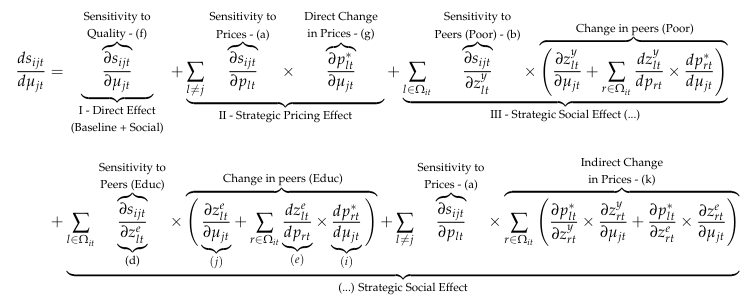
\includegraphics[width=1.05\textwidth, keepaspectratio=true]{figs/quality_markdowns.png}
  \end{center}
\end{frame}
%
\begin{frame}{Quality Markdown}
  \begin{itemize}
  \item Quality and peers are direct substitutes in demand
    \vitem Firms that are better at attracting high SES peers have more market power
    \vitem Term (II) is a result of the two-stage nature of the game
    \vitem Term (III) has two interesting features:
    \begin{itemize}
    \item Strategic social effect on quality reduces strategic incentives to exert market power and reduce quality
      \item Accounts for the screening incentives in the second stage of the pricing game ($a \times k$)
    \end{itemize}
  \end{itemize}
\end{frame}
%
\begin{frame}{Equilibrium}
  A rational-expectations equilibrium is a tuple
  \[
\left\{\left\{\mathbf{z}^{y}, \mathbf{z}^{e}\right\} j \in J,\{\mathbf{p}\} j \in J,\{\boldsymbol{u}\}, j \in J\right\}
  \]
  that satisfies
  \begin{enumerate}
  \item \[
\hat{\mathbf{z}}_{i}^{y}=\mathbf{z}^{y} \text { and } \hat{\mathbf{z}}_{i}^{e}=\mathbf{z}^{e}, \forall i \in I
    \]
  \item \[
p_{j}^{*}\left(\mathbf{p}_{-j}^{*}\right)=\underset{p}{\operatorname{argmax}} \pi_{j}\left(\mu, p, \mathbf{p}_{-j}^{*}, \mathbf{z}^{y}\left(p, \mathbf{p}_{-j}^{*}\right), \mathbf{z}^{e}\left(p, \mathbf{p}_{-j}^{*}\right)\right), \forall j \in J
    \]
  \item \[
     \resizebox{\textwidth}{!}{\mu_{j}^{*}\left(\boldsymbol{\mu}_{-j}^{*}\right)=\underset{\mu}{\operatorname{argmax}} \pi_{j}\left(\mu, \mu_{-j}^{*}, \mathbf{p}^{*}\left(\mu, \mu_{-j}^{*}\right), \mathbf{z}^{y}\left(\mathbf{p}^{*}\left(\mu, \mu_{-j}^{*}\right)\right), \mathbf{z}^{e}\left(\mathbf{p}^{*}\left(\mu, \mu_{-j}^{*}\right)\right)\right)}
    \]
  \end{enumerate}
\end{frame}
%
\begin{frame}{Assumptions}
  \begin{itemize}
  \item Does not model education production function; instead infers MCs from markups and uses these estimated MCs in simulations
    \vitem Counterfactuals must take MC parameters as invariant; cannot address equilibrium effects (e.g. changes in wages)
    \vitem Parameters for student valuations are just weights they place on characteristics, not deep structural preferences
  \end{itemize}
\end{frame}
%
\begin{frame}{Data---Students and Families}
  \begin{enumerate}
  \item Student education data (enrollment and performance)
    \vitem Birth and health records
    \vitem National Household Survey data
    \vitem National Census
    \vitem Scholarship application
  \end{enumerate}
\end{frame}
%
\begin{frame}{Data---Schools}
  \begin{enumerate}
  \item School Characteristics
    \vitem Tuition
    \vitem Teacher data
    \vitem Survey data
    \begin{itemize}
    \item Principals (2016)
    \item Prices (2016)
      \item More prices (2019)
    \end{itemize}
  \end{enumerate}
\end{frame}
%
\begin{frame}{Data---Market Level}
  \begin{enumerate}
  \item National Census (SES characteristics for each market)
    \vitem College graduates
  \end{enumerate}
\end{frame}
%
\begin{frame}{Identification---BLP Instruments}
  \begin{enumerate}
  \item Lagged strike exposure index (2 indexes, distance weighted)
    \vitem Local market strucutre: share of private and number of schools (distance weighted)
    \vitem Local demographics: share high SES (income and education, distance weighted)
  \end{enumerate}
\vfill
Lagged strike exposure should only be coordinated with unions' political factors, which is plausibly excluded from parents' and schools' decisions, but schools with a higher predicted strike probability are more likely to lose students.
\vfill
\end{frame}
%
\begin{frame}{Instruments for price and quality}
  \begin{enumerate}
  \item Public school teacher wage index (distance weighted)
    \vitem Public school teacher vacancies for post-reform contracts (distance weighted)
    \vitem Stock of graduates with education degrees ($t-1$, distance weighted)
    \vitem Test scores for teachers ($t-1$, distance weighted)
    \vitem Flow of new graduates with education degrees to the market
  \end{enumerate}
\end{frame}
%
\begin{frame}{RD to identify price parameters}
  \begin{itemize}
  \item RD around scholarship cutoff
    \vitem Scholarship applicants are probably a selected sample; implement sample correction
    \vitem Use distance to test location as an instrument for scholarship application
  \end{itemize}
\end{frame}
%
\begin{frame}{Estimating Value-Added}
  \[
Y_{i j t}=X_{i t}^{V A} \beta+\theta_{j t}+\epsilon_{i j t}
  \]
  \begin{itemize}
    \item Can estimate by FE or RE
  \vitem Not enough data to include lagged test scores
    \vitem Instead use very, very rich controls for academic results
  \end{itemize}
\end{frame}
%
\begin{frame}{Separating Observable Quality and Peer Effects}
  \begin{itemize}
  \item Estimate $\hat{\theta}_{jt}$ in a first-stage
    \vitem Project $\hat{\theta}_j$ onto peers and inputs, plus a school fixed effect:
    \[
\hat{\theta}_{j t}=\mathbf{z}_{j t}^{\prime} \pi_{j}^{z}+\mathbf{I}_{\mathbf{j t}}^{\prime} \pi^{l}+\alpha_{j}+\epsilon_{j t}
    \]
    \vitem Recover $\mu_{jt}$ by subtracting $z_{jt}(\tau)^\prime \hat{\pi}^z_j$ from $\hat{\theta}_{jt}$
  \end{itemize}
\end{frame}
%
\begin{frame}{Estimation---Parameters }
  Three sets of parameters
  \begin{enumerate}
  \item $\theta_1 = \beta^r$, linear parameters in utility function
    \vitem $\theta_2 = \tilde{\alpha}, \tilde{\beta}^q, \tilde{\beta}^z, \tilde{\beta}^d$, non-linear parameters in utility function
    \vitem $\theta_3 = \gamma$, marginal cost parameter
  \end{enumerate}
\end{frame}
%
\begin{frame}{Estimation---Moments}
  Aggregate moments for shares:
  \[
G^{1}\left(\theta_{2}\right)=s_{j t}^{k}-s_{j t}^{k}\left(\theta_{2}\right)
\]
\vfill
  Micro Moments:
  \[
G_{q}^{2}\left(\theta_{2}\right)=\sum_{i \in N_{k t}^{m}} q_{i k}-\sum_{n}^{N_{m}} \sum_{j}^{N_{m, t}^{f}} s_{j t}^{n k}\left(\theta_{2}\right) \cdot w_{n k}^{m} \cdot q_{j n}
  \]
  \vfill
  Selection Correction for Scholarship Application Moments:
  \[
G^{3}\left(\theta_{2}, \eta\right)=\frac{1}{N_{s}} \nabla_{\eta} \sum_{i} \log \ell_{i}\left(\theta_{2}, \eta\right)
  \]
  \vfill
\end{frame}
%
\begin{frame}{Estimation---Moments}
  Regression Discontinuity Quasi-Experimental Moments:
  \[

\resizebox{\textwidth}{!}{G^{4}\left(\theta_{2}\right)=\frac{1}{N_{s}} \sum_{s=1}^{N_{s}}\left(Z^{\prime}\left(Y_{l}^{s i m}\left(\theta_{2}\right)-X \hat{\beta}_{l}^{R D^{\prime}}\right)\right)^{\prime} W Z^{\prime}\left(Y_{l}^{s i m}\left(\theta_{2}\right)-X \hat{\beta}_{l}^{R D^{\prime}}\right)}
  \]
  \vfill
  IV Moments:
  \[
G^{5}\left(\theta_{2}\right)=\left(\begin{array}{c}
\xi_{j t} \\
\omega_{j t}^{c} \\
\Delta \psi_{j t}
\end{array}\right) \cdot I V^{\prime}
  \]
  \vitem Estimate parameters via GMM according to BLP
\end{frame}
%
\begin{frame}{Results---Peer Effects}
  \begin{center}
    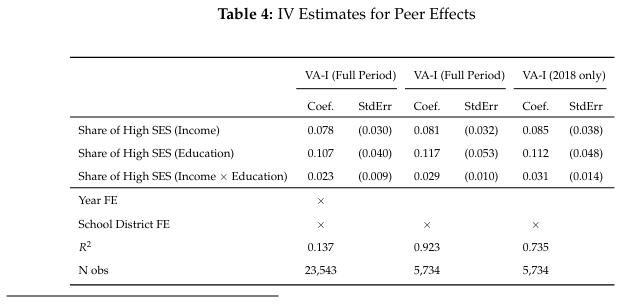
\includegraphics[width=\textwidth, keepaspectratio=true]{figs/tab4.png}
  \end{center}
\end{frame}
%
\begin{frame}{Results---Demand Model}
  \begin{center}
    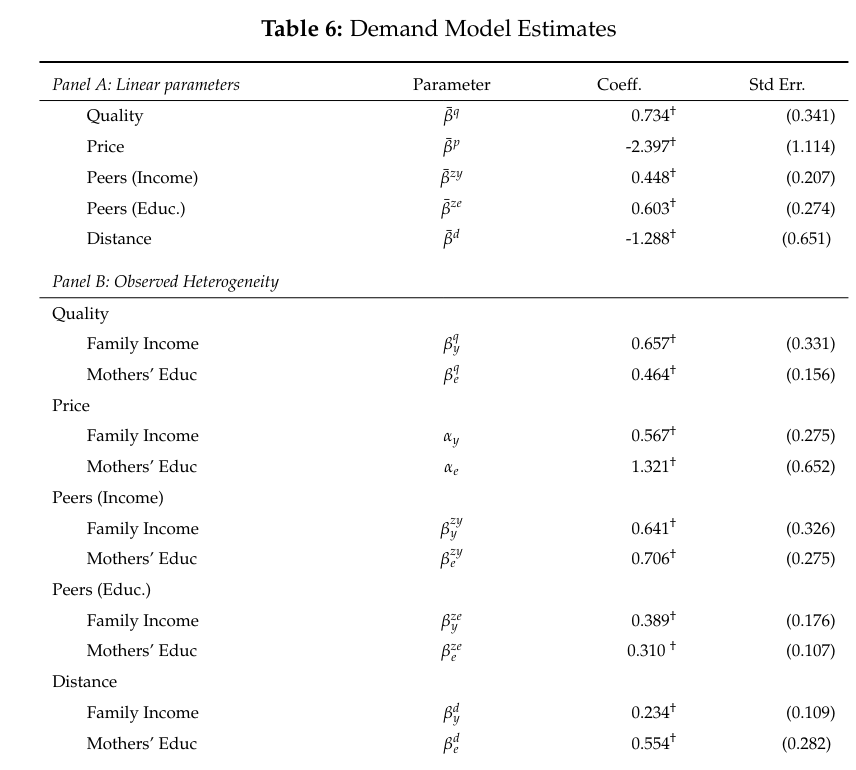
\includegraphics[width=.9\textwidth, keepaspectratio=true]{figs/tab6-1.png}
  \end{center}
\end{frame}
%
\begin{frame}{Results---Demand Model}
  \begin{center}
    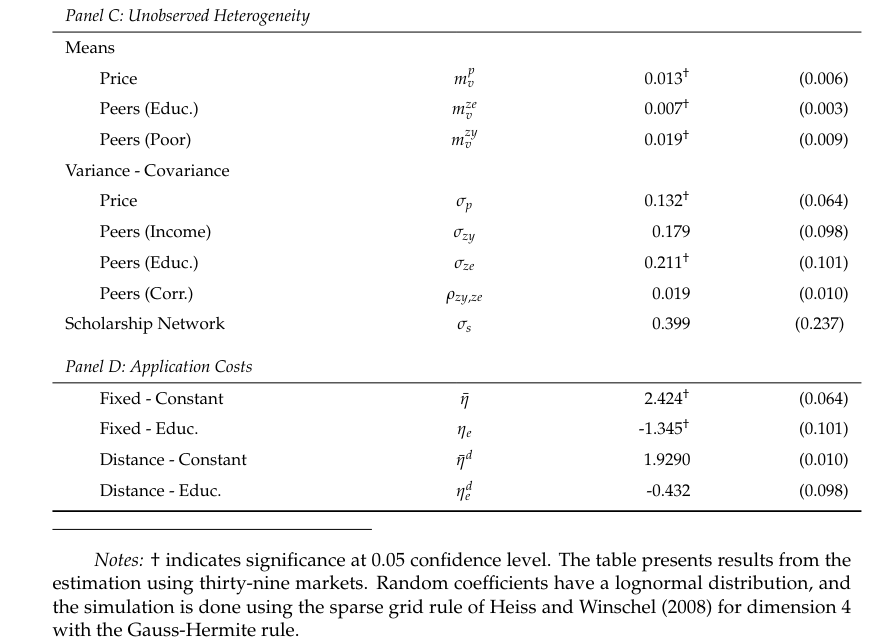
\includegraphics[width=\textwidth, keepaspectratio=true]{figs/tab6-2.png}
  \end{center}
\end{frame}
\begin{frame}{Results---Elasticities and Costs of Quality}
  \begin{center}
    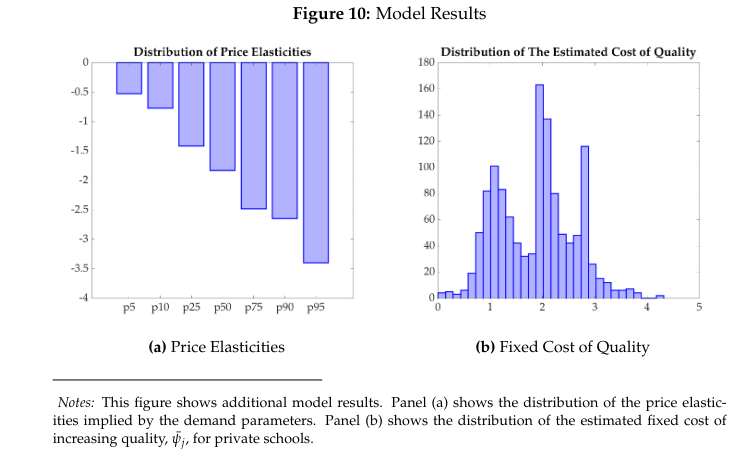
\includegraphics[width=\textwidth, keepaspectratio=true]{figs/fig10.png}
  \end{center}
\end{frame}
%
\begin{frame}{Results---Demand Model}
  \begin{itemize}
  \item These results agree with the theoretical predictions of the model
    \vitem Peers and value-added are direct substitutes in demand
    \vitem Prices are direct complements in demand with peers
    \vitem Prices and peers are strategic complements in demand
  \end{itemize}
\end{frame}
%
\begin{frame}{Counterfactuals}
  \begin{center}
    
\includegraphics[width=\textwidth, keepaspectratio=true]{figs/tab1.png}
  \end{center}
\end{frame}
%
\begin{frame}{Counterfactuals}
  \begin{center}
    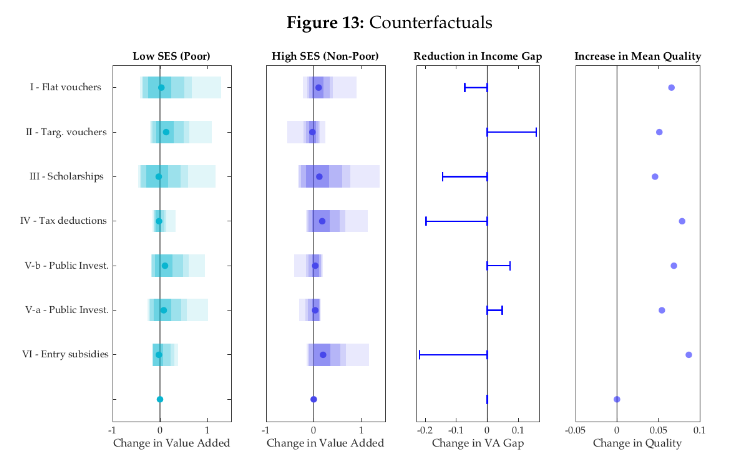
\includegraphics[width=\textwidth, keepaspectratio=true]{figs/fig13.png}
  \end{center}
\end{frame}
%
\begin{frame}{Counterfactuals}
  \begin{center}
    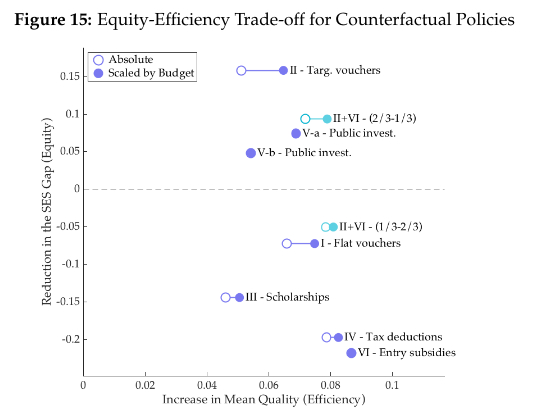
\includegraphics[width=\textwidth, keepaspectratio=true]{figs/fig15.png}
  \end{center}
\end{frame}
%
\begin{frame}{Conclusion/Question}
  \begin{enumerate}
  \item Do you buy the application of BLP to the student/school question?
    \vitem Do you think that including peer effects in this model is a worthwhile contribution?
    \begin{itemize}
    \item Do you think this is the right way to do it?
    \end{itemize}
    \vitem What are other things (in addition to or instead of peer effects) that might be interesting to add?
  \end{enumerate}
\end{frame}
\end{document}
%%% Local Variables:
%%% mode: latex
%%% TeX-master: t
%%% End:
